\chapter{Introduction}

Rare Earth Elements (REEs) play a critical role in modern-day life.
They are used in nearly every device that uses electrical power to operate.
A few examples where REEs are essential are: lasers, computer monitors, electric motors, electric generators, high-power magnets, liquid crystal displays (LCDs), solar panels and many more~\cite{usageofrees}.

\begin{figure}[H]
    \centering
    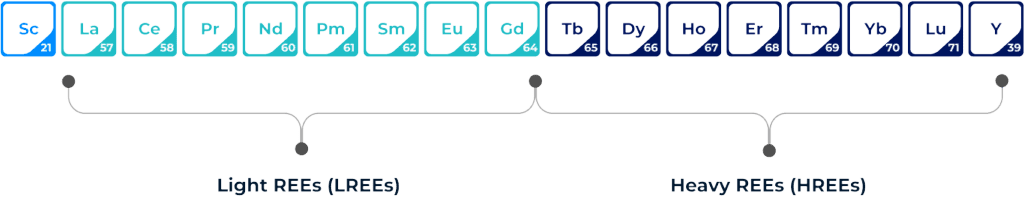
\includegraphics[width=0.9\textwidth]{./media/images/rees_periodic_table}
    \caption{List of all rare earth elements. Those 17 elements can be further categorized into the light rare earth elements (LREEs) and the heavy rare earth elements (HREEs). Picture from REIA / Argus Media.}
    \label{fig:list_rees}
\end{figure}


\section{Problem Setting\authorA{}}

Given the importance of REEs in the modern world, it is evident that the demand for them is increasing quickly.
In the coming years, as the use of electronic devices increases, many of them will become electronic waste.
It is vital for the world's future supply of rare earth elements to recycle them from this waste.

Currently used recycling methods for REEs are mostly damaging to the environment and very costly~\cite{recyclingcurrent}.
Therefore, only around one percent of the global REEs supply is from recycled sources~\cite{currentrecyclingnumbers}.
The rest comes from mining, which brings its own challenges.
Rare earth ores (REOs) often contain radioactive elements which adds more complexity to the processing of the ores.
Also, the extraction of REEs is done by using a process called flotation which produces large amounts of waste water.
This waste water is highly problematic, as it often contains radioactive minerals, acids and toxic agents~\cite{reeenvimpact}.

The processing of REOs does not only damage the environment, but it also contributes to climate change.
As an example, 75 tonnes of \ce{CO2}— equivalents are emitted for every tonne of newly refined neodymium~\cite{reeclimate}.

There are already thousands of tonnes of electronic waste that contain significant amounts of REEs. Recycling them would reduce the need of mining new REOs and therefore reduce the environmental impact of new electronic devices.
Sadly, there is no easy and environmentally friendly process to recycle REEs on an industrial scale.


\section{Contributions\authorB{}}
To combat the issues mentioned above, we worked on a way to recycle REEs without the
need for large amounts of energy or resources.
By using bacteria that produce a special amino acid that allows us to bind the REEs in electronic waste, we achieved just that.
Due to the bacteria not needing significant amounts of energy, we managed to remain eco-friendly and cost-efficient.
The recycling process works by washing shredded electronic waste with our bacteria solution.
After changing the pH value of said solution we can get
the REEs back in their pure forms.
This process works on a scientific level in a laboratory but could also be used on an industrial scale using large bioreactors and washing tanks.


\section{Structure of this Thesis\authorB{}}


